\documentclass[a4paper,11pt]{article}

\usepackage{mlsubmit}
\usepackage{bm}
\usepackage{graphicx}
\begin{document}

\initmlsubmision{2} % assignment number
{Pranjal Nandeshwar}   % your name
{231110035}	% your roll number

\begin{mlsolution}

The objective function in the standard K-means Algorithm is,

\begin{equation}
	\cL(\bm{X}, \bm{Z}, \boldsymbol{\mu}) = \sum_{n=1}^N \sum_{k=1}^K z_{nk} \lVert \bm{x}_n - \bm{\mu}_k \rVert^2
\end{equation}

To make the K-means Algorithm online by taking a random example \(x_n\) at a time,

1) Assign \(x_n\) “greedily” to the “best” cluster.

2) Update the cluster means using SGD on the objective \(\cL\).

For both parts, we need to perform the ALT-OPT Algorithm. To assign \(x_n\) to the best cluster, we need to minimize the objective function by keeping \(\bm{\mu}_k\) as constant.

\textbf{Step 1: Assigning \(x_n\) to the closest cluster}
Fix \(\boldsymbol{\mu} = \hat{\boldsymbol{\mu}}\) and solve for \(z_n\).
\begin{equation}
	\hat{z}_n = \arg\min_{\hat{z}_n} \sum_{k=1}^{K} z_nk \|\mathbf{x}_n - \hat{\boldsymbol{\mu}}_k\|^2 = \arg\min_{\hat{z}_n} z_nk \|\mathbf{x}_n - \hat{\boldsymbol{\mu}}_{\bm{z}_n}\|^2	
\end{equation}

where \(\bm{\mu}_k\) is the mean of the \(k\)-th cluster.

\textbf{Step 2: Updating the cluster means using SGD on the objective \(\cL\)}

The update equation for the mean of cluster \(k\) using stochastic gradient descent (SGD) by fixing \(z = \hat{z}\)

\begin{equation}
	\hat{\bm{\mu}}_k = \arg \min_{\mu_k} \sum_{n:\hat{\bm{z}}_n=k} \|\mathbf{x}_n - \mu_k\|^2.
\end{equation}

At any iteration \(t\), choose an example \(\mathbf{x}_n\) uniformly randomly and approximate \(g\) as
\[
\hat{g}_n = \nabla_{\boldsymbol{\mu}_k} \left(\|\mathbf{x}_n - \boldsymbol{\mu}_k\|^2\right) = -2(\mathbf{x}_n - \boldsymbol{\mu}_k)
\]
Now, the mean can be updated as
\[
\boldsymbol{\mu}_k^{(t+1)} = \boldsymbol{\mu}_k^{(t)} - \eta \hat{g}_n
\]
Therefore,
\[
\boldsymbol{\mu}_k^{(t+1)} = \boldsymbol{\mu}_k^{(t)} + 2\eta (\mathbf{x}_n^{(t)} - \boldsymbol{\mu}_k^{(t)})
\]

\textbf{Choice of step size (\(\eta\)):}
The step size can be chosen as \(\eta \propto \frac{1}{{N_k}}\), where \( N_k \) is the number of data points in the \( k \)-th cluster. This choice ensures that the updated mean is in proportion to the ratio of the sum of features of each data point to the total number of data points in that cluster.

\end{mlsolution}

\begin{mlsolution} 

We want to find projection direction given by $f(\textbf{w})$ vector such that the distances between the means is maximized. Also, we want the inputs within each class to be as close as possible. For this purpose, we have a concept called Linear Discriminant Analysis. Linear Discriminant Analysis maximizes a function $f(\textbf{w})$ that gives a large separation between the class means and also gives small variance within each class. \newline
To implement this concept, we need to maximize the ratio between the "between-class" variance and "within-class" variance. Let us understand the terms: "between-class" variance and "within-class" variance. \newline

1) "Between-class" variance: It means that, the class means must be as far as possible.
For this purpose, we calculate the class means of both the classes.

\begin{equation}
	\boxed{\bm{\hat{\mu}}_+ = \frac{1}{N_+} \sum_{i: y_n = +1}\mathbf{w^T} x_i = \mathbf{w^T\bm{\mu}_+}  }
\end{equation}
\begin{equation}
	\boxed{\bm{\hat{\mu}}_- = \frac{1}{N_-} \sum_{i: y_n = -1}\mathbf{w^T} x_i = \mathbf{w^T\bm{\mu}_-}  }
\end{equation}

Here, $S_b$ is called the scatter between the classes. After calculating the class means, in order to maximize the "Between-class" variance, we need to maximize the following equation,

\begin{equation}
	\boxed{S_b = (\bm{\hat{\mu}}_+ - \bm{\hat{\mu}}_-)^2 }
\end{equation}

2) "Within-class" variance: It means that, the data inputs of a particular class should be as close as possible. To implement this concept, we need to minimize the following equation,
\begin{equation}
	\boxed{S_w = \sum_{i=1}^{N^+} (\textbf{x}_i - \bm{\hat{\mu}}_+)(\textbf{x}_i - \bm{\hat{\mu}}_+)^T + \sum_{i=1}^{N^-} (\textbf{x}_i - \bm{\hat{\mu}}_-)(\textbf{x}_i - \bm{\hat{\mu}}_-)^T}	
\end{equation}
Here, $S_w$ is called the scatter within the class.
The objective function is,
\begin{equation}
\boxed{\bm{J}(w) = \frac{w^T S_w w}{w^T S_b w}}	
\end{equation}
The goal is to find the projection vector $\mathbf{w}$ that maximizes this ratio. By maximizing this ratio, you ensure that the distance between class means becomes as large as possible while keeping the data points within each class as close to each other as possible in the one-dimensional projection.


\end{mlsolution}

\begin{mlsolution}
Suppose we have an eigenvector \(v \in \mathbb{R}^N\) of the matrix \(\frac{1}{N}XX^T\). We can use it to find an eigenvector \(u \in \mathbb{R}^D\) of \(S\), where \(S = \frac{1}{N}X^TX\).

As \(v\) is an eigenvector of \(\frac{1}{N}XX^T\),
\[
\frac{1}{N}XX^Tv = \lambda v
\]

Pre-multiply by \(X^T\), we get,
\[
\frac{1}{N}X^TXX^Tv = \lambda X^Tv
\]

Substitute \(u = X^Tv\), we get,
\[
\frac{1}{N}X^TXu = \lambda u
\]

Now, \(\frac{1}{N}X^TX = S\). Substitute it too,
\[
Su = \lambda u
\]
	This shows that \(u\) is an eigenvector of \(S\) with the same eigenvalue \(\lambda\).


\textbf{Advantage:} The advantage of obtaining eigenvectors of \(S\) in this way is that it allows us to work with a smaller dimensional space. When \(D > N\), directly computing the eigenvectors of \(S\) may be computationally expensive. However, by obtaining the eigenvectors of \(\frac{1}{N}XX^T\) first and then mapping them back to \(S\), we effectively reduce the dimensionality of the problem. This can be particularly useful in situations where computing the eigenvectors is a concern.

\end{mlsolution}

\begin{mlsolution}

\begin{flushleft}
	A conventional linear model is effective when we need to fit a linear curve to the data. However, the versatility of model is limited to linear relationships. In contrast, the proposed model extends its capability by accommodating a combination of $K$ distinct linear curves. Essentially, the model initiates by clustering the data along these $K$ linear curves, and subsequent predictions are then generated for the variable $y$. This approach proves advantageous in handling outliers within a linear curve, as the clustering process may effectively separate and address the impact of outliers.
\end{flushleft}

\begin{flushleft}
	Here, our latent variable model becomes:
\end{flushleft}
\setcounter{equation}{0} % Reset the equation counter
\begin{align}
	p(z_n = k|y_n, \theta) &= \frac{p(z_n = k)p(y_n|z_n = k, \theta)}{\sum_{l=1}^K p(z_n = l)p(y_n|z_n = l, \theta)}
\end{align}
where:
\begin{align}
	p(z_n = k) &= \pi_k 
\end{align}
\begin{align}
	p(y_n|z_n, \theta) &= \mathcal{N}(w_k^T x_n, \sigma^2)
\end{align}

\textbf{ALT-OPT Algorithm}

\textbf{Step 1} Find the best $z_n$:
\begin{align}
	z_n &= \arg\max_{z_n} \frac{\pi_k \mathcal{N}(w_k^T x_n, \sigma^2)}{\sum_{l=1}^K \pi_l \mathcal{N}(w_l^T x_n, \sigma^2)}
\end{align}
which leads to
\begin{align}
	z_n &= \arg\max_{z_n} \frac{\pi_k \exp\left(-\frac{1}{2\sigma^2} (y_n - w_k^T x_n)^2\right)}{\sum_{l=1}^K \pi_l \exp\left(-\frac{1}{2\sigma^2} (y_n - w_l^T x_n)^2\right)}
\end{align}

\textbf{Step 2} Re-estimate the parameters:
\begin{align}
	N_k &= \sum_{n=1}^N z_{nk} \\
	w_k &= (X_k^T X_k)^{-1} X_k^T y_k \\
	\pi_k &= \frac{N_k}{N}
\end{align}
Here, $X_k$ is an $N_k \times D$ matrix containing training sets clustered in class $k$, and $y_k$ are $N_k \times 1$ vectors containing training set labels clustered in class $k$.

If $\pi_k = 1/K$, then:
\begin{align}
	z_n &= \frac{\arg\max_{z_n} \exp\left(-\frac{1}{2\sigma^2} (y_n - w_k^T x_n)^2\right)}{\sum_{l=1}^K \exp\left(-\frac{1}{2\sigma^2} (y_n - w_l^T x_n)^2\right)}
\end{align}

This update is equivalent to multi-output logistic regression.

\end{mlsolution}
	
\begin{mlsolution}

\section{Problem 1}

\subsection{Part 1}
Increasing the regularization hyperparameter leads to an increase in error. This phenomenon is likely because both the training and test sets are derived from the same sine curve without significant outliers. With lower regularization, the model fits the training data more closely, resulting in an indirect improvement in fit for the test data.
\begin{figure} [htb]
	\centering
	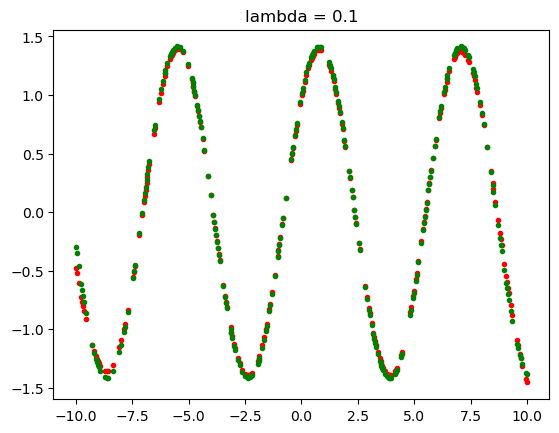
\includegraphics[width=0.5\linewidth]{1.1.png}
	\label{fig:1.1}
\end{figure}
\begin{figure} [htb]
	\centering
	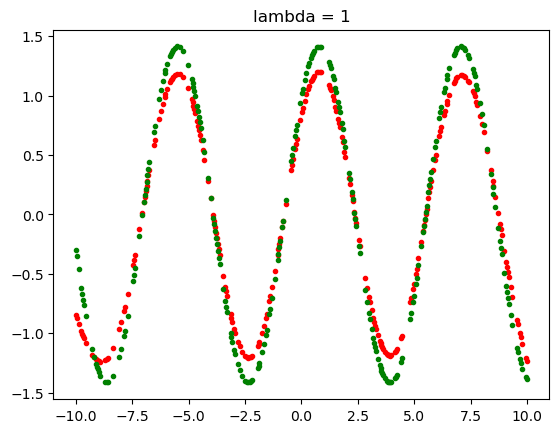
\includegraphics[width=0.5\linewidth]{1.2.png}
	\label{fig:1.2}
\end{figure}
\begin{figure} [htb]
	\centering
	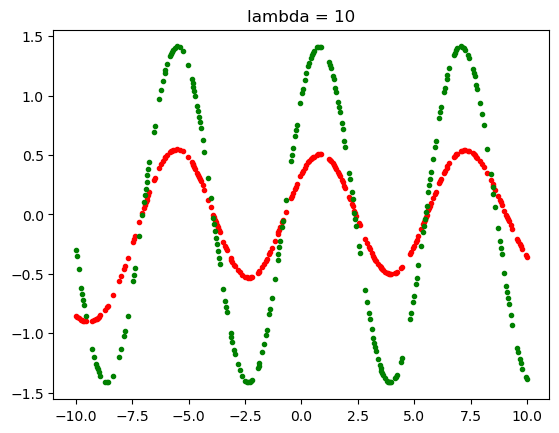
\includegraphics[width=0.5\linewidth]{1.3.png}
	\label{fig:1.3}
\end{figure}
\begin{figure} [htb]
	\centering
	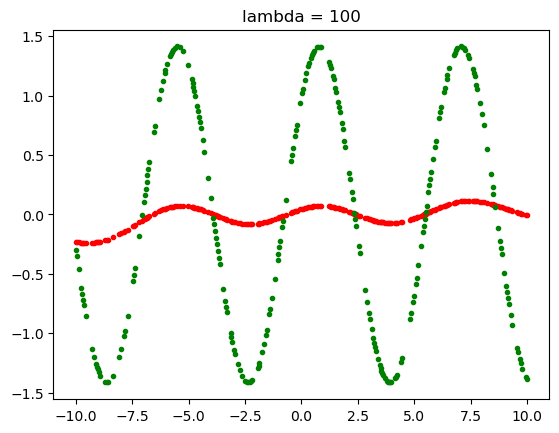
\includegraphics[width=0.5\linewidth]{1.4.png}
	\label{fig:1.4}
\end{figure}
\subsection{Part 2}
A smaller value of \(L\) corresponds to higher prediction errors. This is attributed to fewer feature points being considered. A value of \(L = 50\) is deemed sufficient, as increasing \(L\) to 100 only marginally alters the RMSE by 0.003.
\begin{figure}[h!]
	\centering
	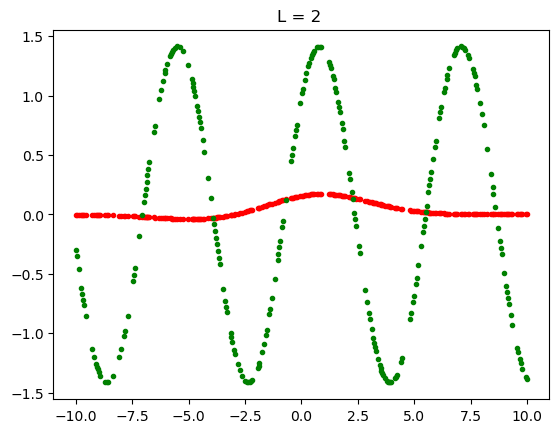
\includegraphics[width=0.5\linewidth]{2.1.png}
	\label{fig:2.1}
\end{figure}
\begin{figure}[h!]
	\centering
	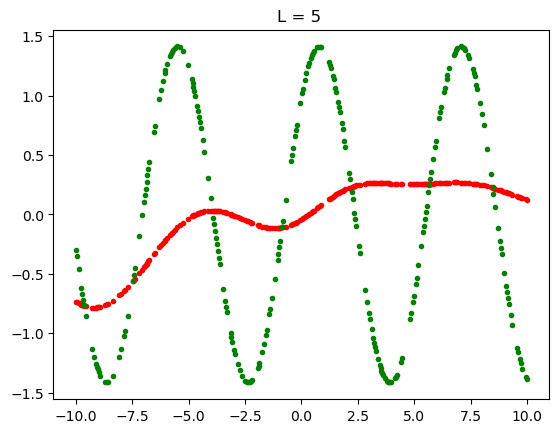
\includegraphics[width=0.5\linewidth]{2.2.png}
	\label{fig:2.2}
\end{figure}
\begin{figure}[h!]
	\centering
	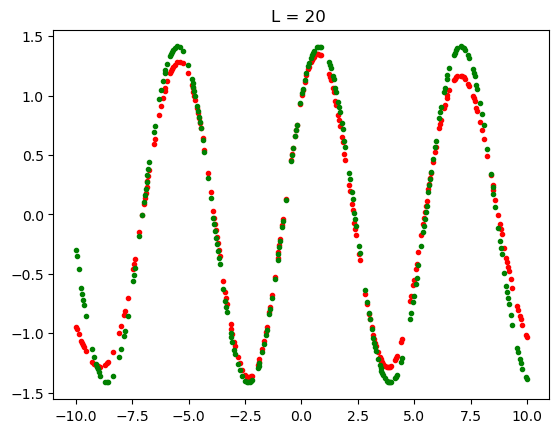
\includegraphics[width=0.5\linewidth]{2.3.png}
	\label{fig:2.3}
\end{figure}
\begin{figure}[h!]
	\centering
	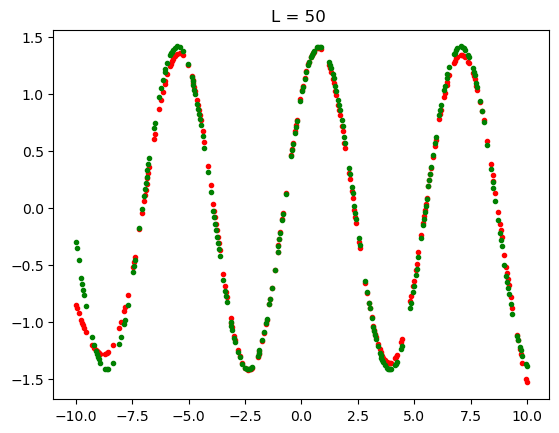
\includegraphics[width=0.5\linewidth]{2.4.png}
	\label{fig:2.4}
\end{figure}

\begin{figure}[H]
	\centering
	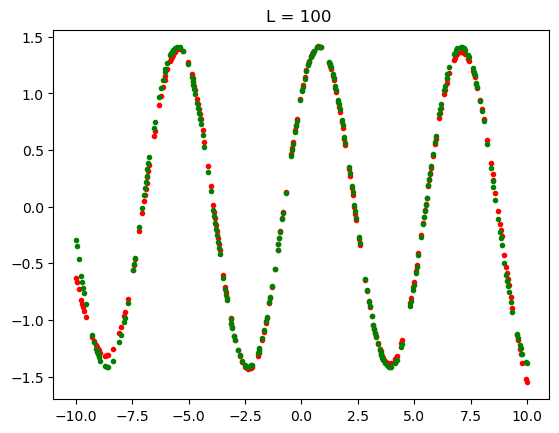
\includegraphics[width=0.5\linewidth]{2.5.png}
	\label{fig:2.5}
\end{figure}
\newpage
\section{Problem 2}

\subsection{Part 1}
After visualizing the data, it becomes evident that the clusters exhibit radial distribution around the origin. Therefore, for the handcrafted part, a feature transformation was employed to represent the distance from the origin.
\begin{figure}[H]
	\centering
	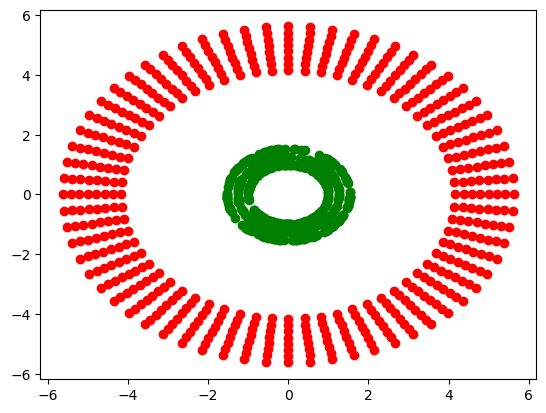
\includegraphics[width=0.5\linewidth]{5.2.1.png}
	\label{fig:5.2.1}
\end{figure}

\subsection{Part 2}
Effective clustering of the given data can be achieved through a feature transformation based on the distance of each point from the origin. The choice of a landmark significantly influences clustering success, particularly when the selected landmark is in proximity to the origin. However, if the landmark is distant from the origin, clustering effectiveness diminishes, given the radial distribution of data around the origin.
\begin{figure}[H]
	\centering
	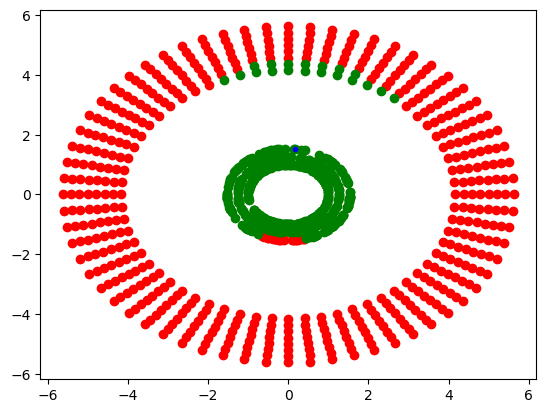
\includegraphics[width=0.5\linewidth]{5.2.2.1.png}
	\label{fig:5.2.2.1}
\end{figure}
\begin{figure}[H]
	\centering
	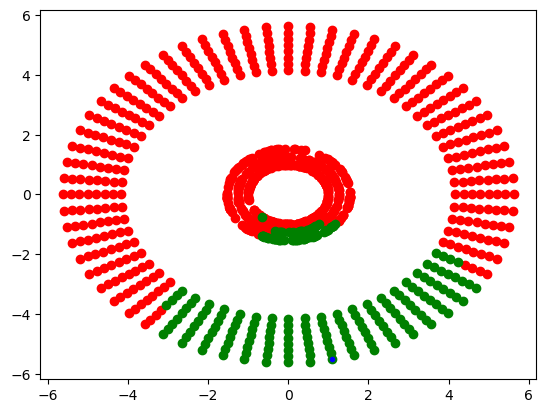
\includegraphics[width=0.5\linewidth]{5.2.2.2.png}
	\label{fig:5.2.2.2}
\end{figure}
\begin{figure}[H]
	\centering
	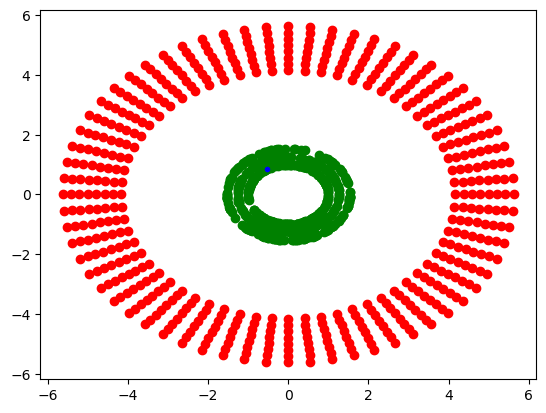
\includegraphics[width=0.5\linewidth]{5.2.2.3.png}
	\label{fig:5.2.2.3}
\end{figure}
\begin{figure}[H]
	\centering
	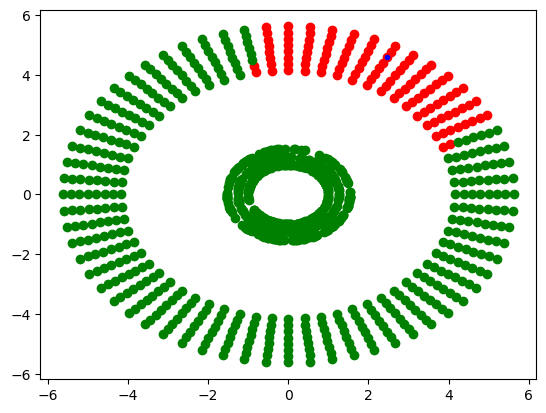
\includegraphics[width=0.5\linewidth]{5.2.2.4.png}
	\label{fig:5.2.2.4}
\end{figure}
\begin{figure}[H]
	\centering
	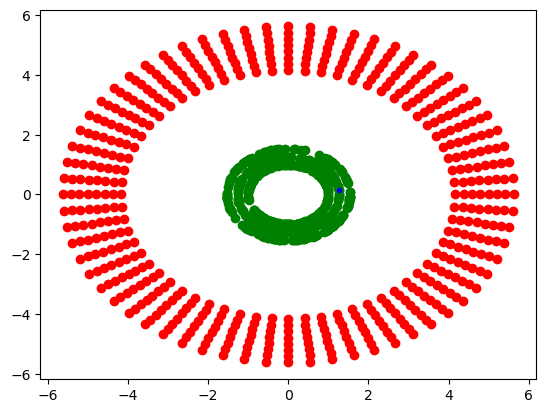
\includegraphics[width=0.5\linewidth]{5.2.2.5.png}
	\label{fig:5.2.2.5}
\end{figure}
\begin{figure}[H]
	\centering
	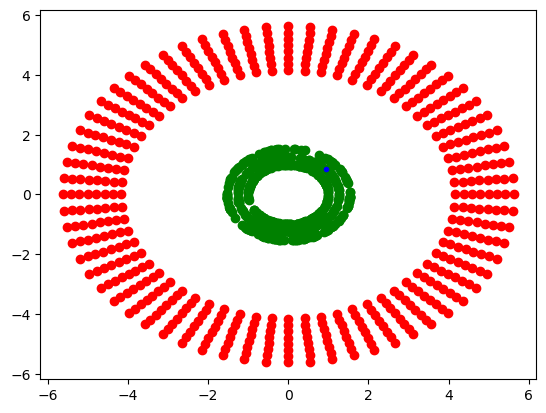
\includegraphics[width=0.5\linewidth]{5.2.2.6.png}
	\label{fig:5.2.2.6}
\end{figure}
\begin{figure}[H]
	\centering
	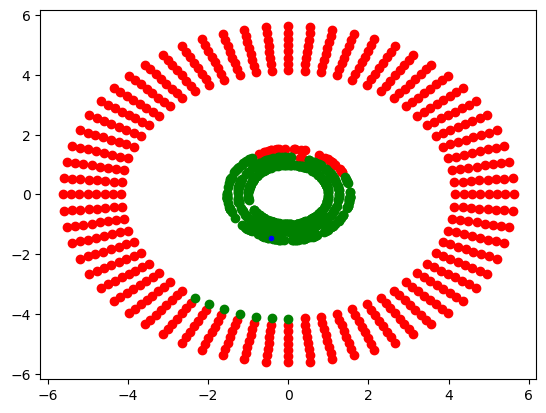
\includegraphics[width=0.5\linewidth]{5.2.2.7.png}
	\label{fig:5.2.2.7}
\end{figure}
\begin{figure}[H]
	\centering
	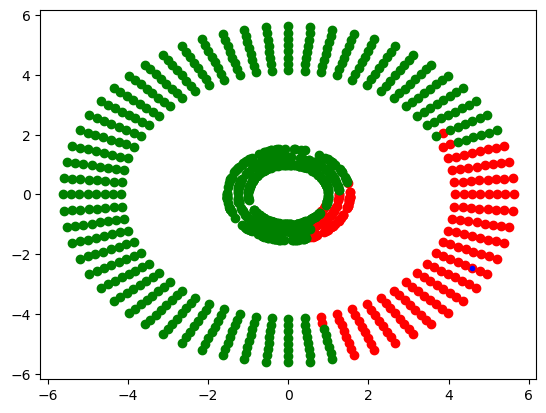
\includegraphics[width=0.5\linewidth]{5.2.2.8.png}
	\label{fig:5.2.2.8}
\end{figure}
\begin{figure}[H]
	\centering
	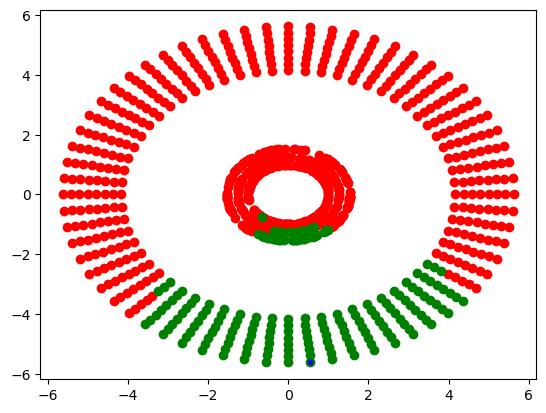
\includegraphics[width=0.5\linewidth]{5.2.2.9.png}
	\label{fig:5.2.2.9}
\end{figure}
\begin{figure}[H]
	\centering
	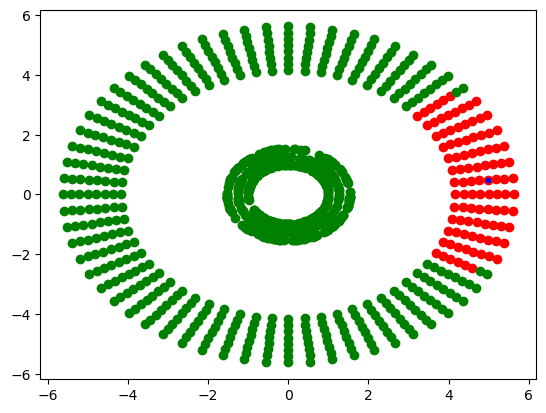
\includegraphics[width=0.5\linewidth]{5.2.2.10.png}
	\label{fig:5.2.2.10}
\end{figure}

\newpage
\section{Problem 3}

The difference between PCA and t-SNE plots lies in their ability to capture different aspects of the data's structure. While PCA emphasizes global structures, t-SNE excels at preserving local similarities and patterns in the data. In t-SNE plots, distinct clusters and class separations are more visible, making it particularly effective for visualizing high-dimensional data with complex relationships. Conversely, PCA plots may exhibit more overlap between classes and focuses on the global structure of the data.
\begin{figure}[H]
	\centering
	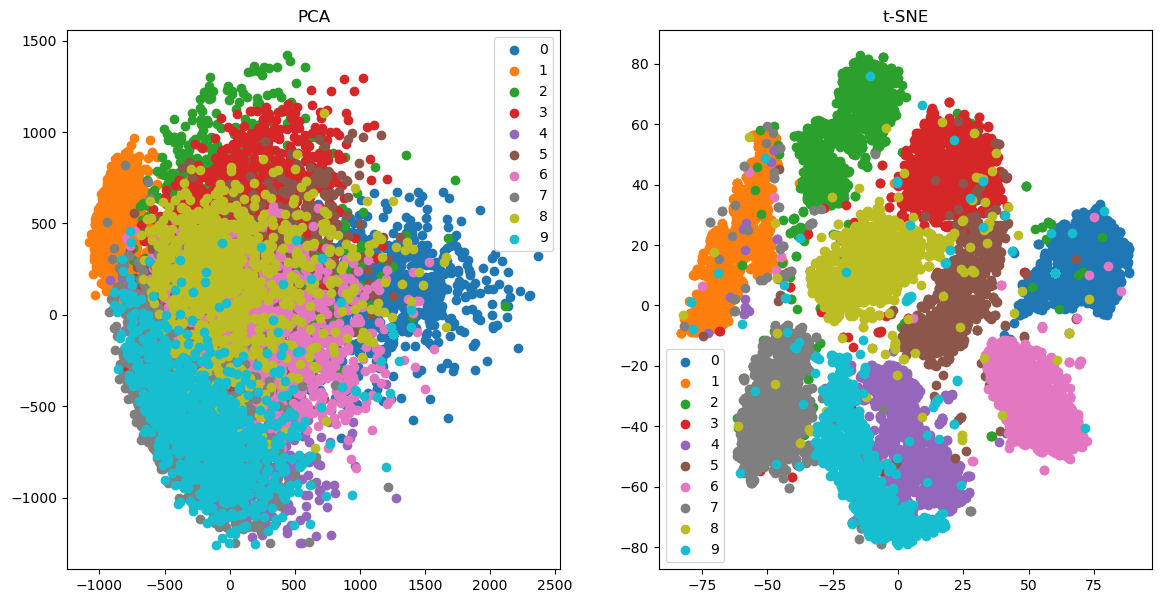
\includegraphics[width=1\linewidth]{3.1.png}
	\label{fig:3.1}
\end{figure}
\end{mlsolution}

\end{document}
